\section{从幂迭代到 QR 特征值算法}
\label{sec:08-Numerical-Analysis/05-Numerical-Linear-Algebra/05}

一张两千万节点的关系图摆在面前，任务不是解方程，而是拿到它的主特征向量：排序要用它，聚类前的谱嵌入也要用它。矩阵存成稀疏格式，一次矩阵--向量乘几十毫秒；分解它则想都不用想。上一节把 Krylov 子空间当成解线性系统的工具，这一节要问的是同一组向量里的另一半信息——谱。

先从最朴素的做法开始：取一个向量，反复乘 \(A\)，看会浮出什么。

\subsection{反复相乘会让主特征方向胜出}

设 \(A\) 实可对角化，特征值按模长排开，\(x_0=\sum_i c_i v_i\) 在主方向上有分量。乘 \(k\) 次：

\[
A^kx_0=\lambda_1^k\Bigl[c_1v_1+\sum_{i>1}c_i\Bigl(\frac{\lambda_i}{\lambda_1}\Bigr)^{k}v_i\Bigr].
\]

括号里除第一项外，每一项每乘一次就被压缩 \(\abs{\lambda_i/\lambda_1}\) 倍。主方向什么都没做，只是别的方向都在退场，它就赢了。模长会指数爆炸或塌缩，所以每步归一化，这就是幂迭代：

\[
y_{k+1}=Ax_k,\qquad x_{k+1}=\frac{y_{k+1}}{\norm{y_{k+1}}_2}.
\]

条件对账值得逐条走：要求 \(A\) 可对角化，否则展开式不成立（Jordan 块会让收敛退化成 \(k\) 的多项式因子）；要求 \(\abs{\lambda_1}>\abs{\lambda_2}\) 严格成立，否则前两个方向谁也压不倒谁；要求 \(c_1\neq0\)，随机初值以概率 1 满足，但浮点下若 \(c_1\) 极小，前若干步会看上去停滞；\(\lambda_1\) 为负时向量每步翻号，为复数时带着相位转，方向不收敛而二维不变子空间仍收敛。

收敛速度写在一个比值上：\(\abs{\lambda_2/\lambda_1}\)。它是 0.4 还是 0.99，决定了这个算法是三步就完事还是跑上几千步。

\begin{center}
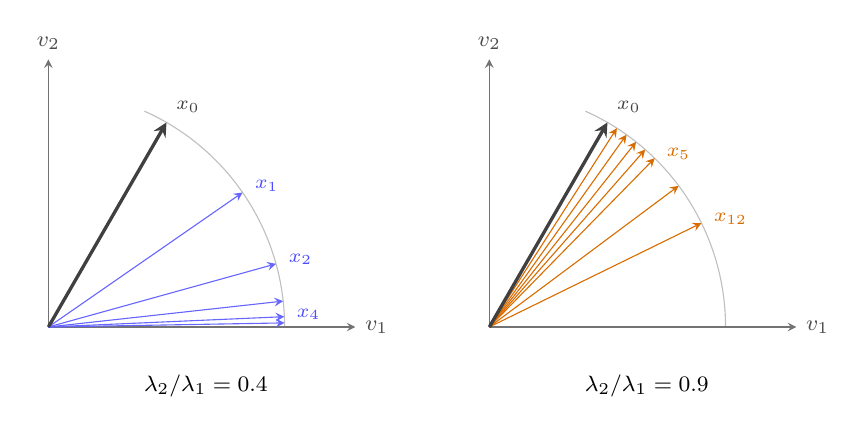
\begin{tikzpicture}[font=\small,>=stealth]
  \begin{scope}
    \draw[black!25] (3,0) arc (0:66:3);
    \draw[->,black!55] (0,0) -- (3.9,0);
    \draw[->,black!55] (0,0) -- (0,3.4);
    \node[right,font=\footnotesize,black!70] at (3.9,0) {\(v_1\)};
    \node[above,font=\footnotesize,black!70] at (0,3.4) {\(v_2\)};
    \foreach \dx/\dy in {2.466/1.708, 2.891/0.802, 2.982/0.329, 2.997/0.131, 3.000/0.052}{
      \draw[->,blue!60] (0,0) -- (\dx,\dy);}
    \draw[->,very thick,black!75] (0,0) -- (1.500,2.598);
    \node[above right,font=\scriptsize,black!75] at (1.500,2.598) {\(x_0\)};
    \node[right,font=\scriptsize,blue!70] at (2.50,1.79) {\(x_1\)};
    \node[right,font=\scriptsize,blue!70] at (2.93,0.86) {\(x_2\)};
    \node[right,font=\scriptsize,blue!70] at (3.03,0.16) {\(x_4\)};
    \node[font=\footnotesize] at (2.0,-0.75) {\(\abs{\lambda_2/\lambda_1}=0.4\)};
  \end{scope}
  \begin{scope}[shift={(5.6,0)}]
    \draw[black!25] (3,0) arc (0:66:3);
    \draw[->,black!55] (0,0) -- (3.9,0);
    \draw[->,black!55] (0,0) -- (0,3.4);
    \node[right,font=\footnotesize,black!70] at (3.9,0) {\(v_1\)};
    \node[above,font=\footnotesize,black!70] at (0,3.4) {\(v_2\)};
    \foreach \dx/\dy in {1.620/2.525, 1.742/2.442, 1.864/2.351, 1.980/2.254,
                         2.100/2.144, 2.405/1.793, 2.694/1.320}{
      \draw[->,orange!85!black] (0,0) -- (\dx,\dy);}
    \draw[->,very thick,black!75] (0,0) -- (1.500,2.598);
    \node[above right,font=\scriptsize,black!75] at (1.500,2.598) {\(x_0\)};
    \node[right,font=\scriptsize,orange!85!black] at (2.13,2.20) {\(x_5\)};
    \node[right,font=\scriptsize,orange!85!black] at (2.73,1.37) {\(x_{12}\)};
    \node[font=\footnotesize] at (2.0,-0.75) {\(\abs{\lambda_2/\lambda_1}=0.9\)};
  \end{scope}
\end{tikzpicture}

\emph{同一个初值、同一套迭代，比值 0.4 时四步就贴上了主方向，比值 0.9 时十二步还差着二十多度——幂迭代的成本不由矩阵多大决定，由谱间隙决定。}
\end{center}

图里两块画的是同一个算法。左边那种情形，你写的代码好不好几乎无所谓；右边那种，任何常数因子的优化都救不了，只有换算法或者动谱本身。

特征值的估计用 Rayleigh 商 \(\rho(x)=x^{\trans}Ax/(x^{\trans}x)\)。对称情形下它有二次精度：方向误差是 \(\theta\) 时，特征值误差是 \(O(\theta^2)\)。也正因为如此，拿 Rayleigh 商的变化量当停止判据会上当——方向还在缓慢漂移，商却早已看起来收敛。该看的是特征残差 \(\norm{Ax-\rho(x)x}_2\)。

\subsection{特征多项式在数值上不是求特征值的方法}

如果你还记得课本，第一反应大概是解 \(\det(A-\lambda I)=0\)：展开行列式得到 \(n\) 次多项式，再求根。纸上 \(n=3\) 时没问题，浮点下这条路第一步就废了。

原因是多项式的根对系数极端敏感。把系数 \(a_j\) 扰动 \(\delta\)，根 \(\lambda\) 的一阶位移是

\[
\Delta\lambda\approx-\,\delta\,\frac{\lambda^{j}}{p'(\lambda)},
\qquad
p'(\lambda)=\prod_{i\colon\lambda_i\neq\lambda}(\lambda-\lambda_i).
\]

分子是根的高次幂，分母是它到其余各根的距离之积。根稍微密集一点，分母就小得可怕；根稍微大于 1，分子就大得可怕。Wilkinson 多项式 \(p(x)=(x-1)(x-2)\cdots(x-20)\) 把两头同时占满：在 \(\lambda=15\) 处，\(\abs{15^{19}/p'(15)}\approx2\times10^{9}\)。给 \(x^{19}\) 的系数加上 \(2^{-23}\) 这么一点扰动，若干个实根就成对变成复数。一阶估计会高估实际位移，但量级已经说明问题：从矩阵到系数这一步先放大一次误差，从系数到根再放大一次，最后拿到的数字与真实特征值没有关系。

反过来看更有意思。\texttt{numpy.roots} 求多项式根的做法，是构造伴随矩阵再调用特征值例程——业界公认的方向是从多项式走向矩阵，不是从矩阵走向多项式。

于是现代算法走另一条路：对矩阵反复做正交相似变换，把它推到能直接读出特征值的形状。正交变换保谱，且二范数条件数恒为 1，误差不会在过程中被放大。

\subsection{位移把小间隙翻成大间隙}

要找的若不是最大特征值，而是离某个给定值 \(\sigma\) 最近的那个，就对 \((A-\sigma I)^{-1}\) 做幂迭代。它的特征值是 \(1/(\lambda_i-\sigma)\)：原来最难分辨的那个小间隙，取倒数后成了压倒性的最大模。代价是每步要解 \((A-\sigma I)y=x_k\)，通常先对 \(A-\sigma I\) 做一次 LU，之后每步只需 \(O(n^2)\) 的回代；同一位移下迭代得越多，那次 \(O(n^3)\) 分解摊得越薄。

把 \(\sigma\) 换成当前的 Rayleigh 商，每步都用最新估计重新定位，就得到 Rayleigh 商迭代，对称情形下收敛是三次的。它每步都要重新分解，而且逼近的是哪个特征值取决于初值，不受控制。

\subsection{一组正交基同时做幂迭代，就是 QR 迭代}

幂迭代只看得见一个方向。想要前 \(p\) 个，自然的做法是让 \(p\) 个向量同时迭代；但它们会一起坍缩到主方向，所以每步乘完 \(A\) 之后重新正交化。这就是子空间迭代，而它的紧凑写法正是 QR 迭代：

\[
A_k=Q_kR_k,\qquad A_{k+1}=R_kQ_k.
\]

分解再反乘，这一行为什么有意义？因为 \(R_k=Q_k^{\trans}A_k\)，代回去得到

\[
A_{k+1}=Q_k^{\trans}A_kQ_k,
\]

每一步是正交相似变换，谱一个不少。适当条件下 \(A_k\) 趋向上三角的 Schur 形（实矩阵是准上三角，复共轭对留在 \(2\times2\) 块里），特征值就排在对角上。QR 迭代不是与幂迭代无关的新想法，它是幂迭代搬到一组正交基上之后的组织方式。

从这一行到能跑的软件之间还隔着三件工程。第一件是 Hessenberg 约化：用 Householder 相似变换把 \(A\) 化为次对角线以下全零的形状（对称时化为三对角），这是一次性的 \(O(n^3)\)；此后每步 QR 只需消掉次对角线上 \(n-1\) 个元素，单步成本从 \(O(n^3)\) 降到 \(O(n^2)\)。第二件是带位移的隐式扫描：位移让迭代实际作用在 \(A_k-\mu I\) 上再加回 \(\mu I\)，效果与 shift-invert 同源，右下角元素因此衰减极快；所谓隐式，是指位移通过第一个 Householder 反射器嵌进去，不必真的减去再加回，从而避免了 \(\mu\) 接近某个特征值时的相消。第三件是 deflation：某个次对角元小到与邻元的机器精度尺度相当时，就把它当零，问题拆成两个更小的子问题。对称三对角情形配 Wilkinson 位移（取右下角 \(2\times2\) 块中更靠近角元的那个特征值），实践中几乎总是三步以内收敛一个特征值——LAPACK 的对称特征值例程走的就是这条线。

规模再大一层，连 \(O(n^2)\) 的扫描也不划算，这时回到 Krylov：Lanczos（对称）与 Arnoldi（一般）在 \(\operatorname{span}\set{b,Ab,A^2b,\ldots}\) 上建正交基，把特征问题投影到一个几十维的小矩阵上再用稠密算法解。上一节用同一组基逼近解，这一节用它逼近谱，两件事共用同一次矩阵--向量乘。

\subsection{PageRank 把收敛率变成了一个产品参数}

\hyperref[sec:06-Random-Processes/04-Applications/03]{``PageRank：把网页排序变成平稳概率''}给出的评分向量 \(p\) 满足 \(Pp=p\)，即 \(P\) 对应特征值 1 的特征向量。从随机概率向量出发反复算 \(p_{k+1}=Pp_k\)，就是一次幂迭代，而 \(n\) 可能上百亿。

这里 \(\lambda_1=1\) 是确定的，所以全部悬念落在 \(\abs{\lambda_2}\) 上。网络里若存在几乎互不链接的大社区，\(\abs{\lambda_2}\) 就贴近 1，迭代次数随之失控——这不是工程能优化掉的，是谱结构本身。PageRank 的做法是把转移矩阵换成

\[
P_\alpha=(1-\alpha)P+\alpha\,\tfrac1n\ind\ind^{\trans},
\]

随机跳转一次性解决了悬挂节点、周期性和收敛速度三件事，第二大特征值的模被压到 \(1-\alpha\) 以下，\(\alpha=0.15\) 时约五十步就能到工程精度。但它同时挪动了稳态的定义：\(\alpha\) 不是一个纯数值旋钮，调它等于改了``重要性''的含义。谱聚类里也是同一件事，那里关心的是 Laplacian 最小的那几个特征值，间隙大小直接对应簇分得开不开。

\subsection{对称矩阵和非正规矩阵不是同一道题}

对称矩阵的特征值是良态的：特征向量系正交，条件数为 1，Weyl 定理给出 \(\abs{\lambda_i(A+E)-\lambda_i(A)}\le\norm{E}_2\)，扰动不会被放大。这也是\hyperref[ch:020]{``特征值、对角化与动力系统''}里那套几何图像能直接搬到浮点上的原因。

非正规矩阵不同。取

\[
A=\begin{pmatrix}1&M\\0&1+\varepsilon\end{pmatrix},
\]

特征值是 \(1\) 与 \(1+\varepsilon\)，看着分离良好，但 \(M\) 大而 \(\varepsilon\) 小时两个特征向量几乎平行，矩阵逼近缺陷。加一个大小为 \(\delta\) 的扰动，特征值可以移动 \(\sqrt{M\delta}\) 量级，远超 \(\delta\)。糟糕的是残差 \(\norm{Av-\lambda v}_2\) 此时仍可能很小——后向误差合格，前向误差却离谱，\hyperref[sec:08-Numerical-Analysis/01-Floating-Point-and-Error/04]{``前向误差、后向误差与稳定算法''}里那笔账在谱问题上原样重演。对这类矩阵，报告不变子空间比报告单个特征向量诚实，Schur 分解给的正是正交不变子空间；若要量化敏感性，伪谱（对每个 \(\varepsilon\) 标出满足 \(\norm{(zI-A)^{-1}}_2\ge1/\varepsilon\) 的全部 \(z\)）比单个条件数说得清楚。

\subsection{先问需要多少谱信息，再选算法}

三个问题就能定下方案。矩阵对称吗——对称就用保结构的路径，不要用通用例程把结构丢掉。要全部特征值还是前几个——全部就老实做稠密 QR，\(O(n^3)\)；只要 \(k\ll n\) 个极端特征值，Krylov 或随机化子空间迭代的代价由矩阵--向量乘主导，量级降到 \(O(n^2k)\) 甚至更低。矩阵稀疏吗——稀疏时 matvec 极快，而稠密算法的 Hessenberg 约化会立刻把稀疏性填满，两者不能混用。

随机化方法在超大规模上给了第三条路：用一个 \(n\times(k+p)\) 的随机矩阵 \(\Omega\) 一次性打出草图 \(Y=A\Omega\)，对 \(Y\) 做 QR 取正交基 \(Q\)，把问题压成 \(B=Q^{\trans}AQ\) 再用稠密算法解。它有效的原因和幂迭代同源：随机向量在所有特征方向上都有分量，主方向被捕获的概率接近 1，过采样余量 \(p\) 取 5 到 10 就够。但它是筛选工具而不是精加工工具——谱衰减慢时草图捕不住尾部，结果还需要 Rayleigh--Ritz 细化。

到这里，特征值这条线已经从最朴素的重复相乘走到了生产级软件。下一节换一类分解：不再要求矩阵是方阵，也不再问它有什么不变方向，只问它把哪些方向放大、哪些方向几乎压成零——以及当``几乎''小到和舍入误差同一量级时，秩这个词还剩下什么含义。
